% !TeX program = xelatex
% !TeX encoding = UTF-8
\documentclass[UTF8]{standalone}
\usepackage{amsmath,newtxmath,ctex,tikz}
\begin{document}
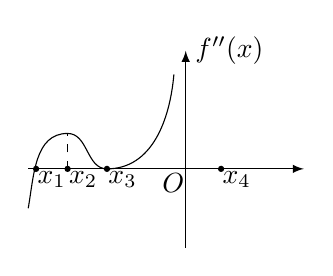
\begin{tikzpicture}
	\draw[domain=0.18:1.3,smooth,samples=100]  plot[id=1] function{log(x)+0.8};
	\draw[-latex] (-2,0) -- ++ (3.5,0);
	\draw[-latex] (0,-1) -- ++ (0,2.5) node[right] {$f''(x)$};
	\fill (0.4493289,0) circle (0.04) node[below=4pt,right=-3pt] {$x_4$};
	\fill (-1,0) circle (0.04) node[below=4pt,right=-3pt] {$x_3$};
	\fill (-1.5,0) circle (0.04) node[below=4pt,right=-3pt] (a) {$x_2$};
	\draw[dashed] (-1.5,0) -- (-1.5,0.45);
	\fill (-1.9,0) circle (0.04) node[below=4pt,right=-3pt] {$x_1$};
	\node[below=5pt,left=-3pt] at (0,0) {$O$};
	\draw (-2,-0.5) to[out=80,in=-180] (-1.5,0.45);
	\draw (-1.5,0.45) to[out=0,in=-180] (-1,0);
	\draw (-1,0) to[out=0,in=-95] (-0.15,1.2);
\end{tikzpicture}
\end{document}